\chapter{Detecting corruption, collusion \& fraud: Data product}\label{chap_product}


This chapter first describes the details in the modeling process for the identification of possible cases of corruption, collusion and fraud within the World Bank's Major and Historical awards and investigations data. After that, this chapter explains  how does the visualization created for the World Bank's investigation team in the Integrity Vice Presidency works. Section \ref{sec_pipeline} is visualization of the data pipeline that sustains the web application that runs in the Wolrd Bank's servers. Section \ref{sec_models} gives the details of the model selected for the identification of corruption, collusion and fraud and finally, section \ref{sec_visual} shows the different visualizations made for a more proactive investigation process.

\section{Data pipeline} \label{sec_pipeline}

As chapter \ref{chap_data} shows, there are different data sources, figure \ref{fig_pipeline} shows a summary of how the data from all the sources was combined into a web application that runs in the server of the World Bank and helps the investigators at the Integrity Vice Presidency to investigate projects and entities in a more proactive way than by relying on whistle-blowers. Figure \ref{fig_pipeline} shows how the different data sources first combine into the Google Algorithm for name disambiguation explained on chapter \ref{chap_data}. Then the resulting tables are joined with the World Bank's Development indicators for each country. After this, all the country specific and co-award network features explained in section \ref{sec_features} were produced so that finally everything feeds the model that can potentially identify malicious contracts or contractors.

\begin{figure}[H]
\begin{center}
\caption{Data pipeline}
\label{fig_pipeline}
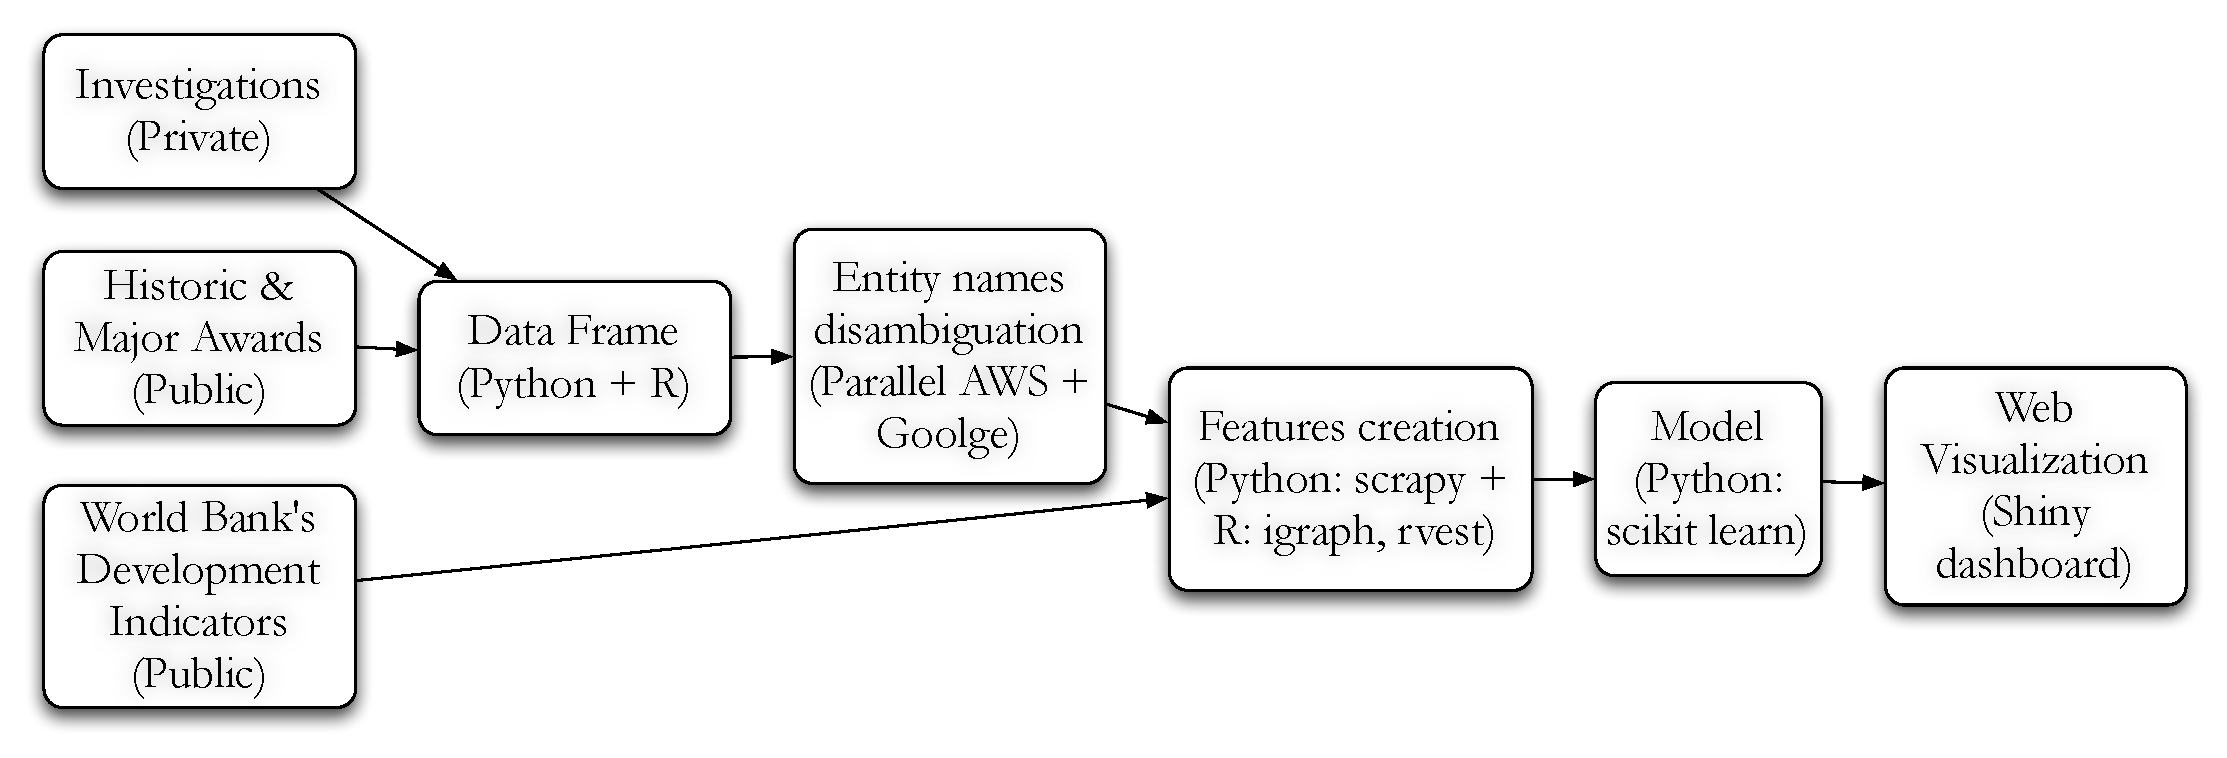
\includegraphics[width=\textwidth,height=1\textheight,keepaspectratio]{../img/pipeline.pdf}
\end{center}
\noindent \footnotesize{\textbf{Source:} Own creation.}
\end{figure}

The steps illustrated  in figure \ref{fig_pipeline} were explained in previous chapters up to the feature creation. The next sections cover the modeling and the visualizations.

\section{Model} \label{sec_models}

As the introduction says in page \pageref{dssg} any Data Science project such as this one requires a solvable problem, that is challenging, has impact, has relevant data and committed partner. Up to this face we have stated that detecting corruption, collusion and fraud  is challenging enough, the Google searches algorithm and the co-awards network is a clear example of that. The impact was stated in figures such as \ref{fig_major_awarded_usd} that shows the amount that the World Bank gives in its procurements contracts in its effort to reduce global poverty. It more than enough and relevant data  from different sources that complement to each other and a clearly committed partner. Up to this point the project is just missing a solution to identification of corruption, collusion and fraud such that it becomes a solvable problem.  

We needed to create a solvable problem within the time restrictions stated at the time of the project. Unfortunately, the most relevant data came way after the project started and the name disambiguation algorithm took long enough to have long enough time for the next steps of the project, which was, the modeling step. The idea is to find a model that is able to identify potential cases of corruption, collusion or fraud within the World Bank's data. 

A traditional modeling process like this involves comparing different approaches in order to minimize the desired error or maximize the accuracy of a classification or prediction.


For this project, three different models were considered, a classifier  using a Supported Vector Machine (SVM), a Random Forest and a Logistic Regression. To evaluate the output we created the dependent variable by considering the labels in the investigations data by labeling any substantiated case as guilty and not guilty in any other case. See \cite{hasti} for more details on SVM, random forest and logistic regression. 


To select the models first we took a training set from the data by sorting by date so that the data for the past would be able to identify potential corruption, collusion and fraud in the data for the future relative to the training data. To select the parameters of each model we used some crossed validation in terms of the Area Under Curve (AUC) of the Receiver Operating Characteristic curve (ROC), ROC-AUC. See \ref{chap_code} and the code \ref{code_models} to see how the parameters of the models were selected.

Since all the investigations data was private, unfortunately for this paper,  the modeling phase cannot be replicated because of the access to the data so the paper cannot show the results of the different models tunned. Nevertheless, after tunning with different parameters and considering different features, the resulting model was a Random Forest which has a ROC curve that can be seen at figure \ref{fig_roc}. The figure \ref{fig_roc} contains the percentage of the  investigated and not guilty contracts that were marked  by the model as ``should be investigated'' (false positive rate) against the percentage of investigated contracts caught by the model (true positive rate).The figure shows in green the ROC curve for the random forest considering the co-awards network features and the blue curve refers to the ROC without the co-awards network features. As it can be seen from the figure, the network features add accuracy to the prediction so they are very desirable for the World Bank Investigators.

It is also important to notice here that the random forest is a great model for the investigators at the Integrity Vice Presidency because it is a much better classifier than the actual benchmark which was just guessing whether they should investigate a contract, entity or project or not. The dashed line in figure \ref{fig_roc} represents a random guess, so the farther the ROC curve is from that line, the better the quality of the classification.

\begin{figure}[H]
\begin{center}
\caption{ROC: Random forest test data}
\label{fig_roc}
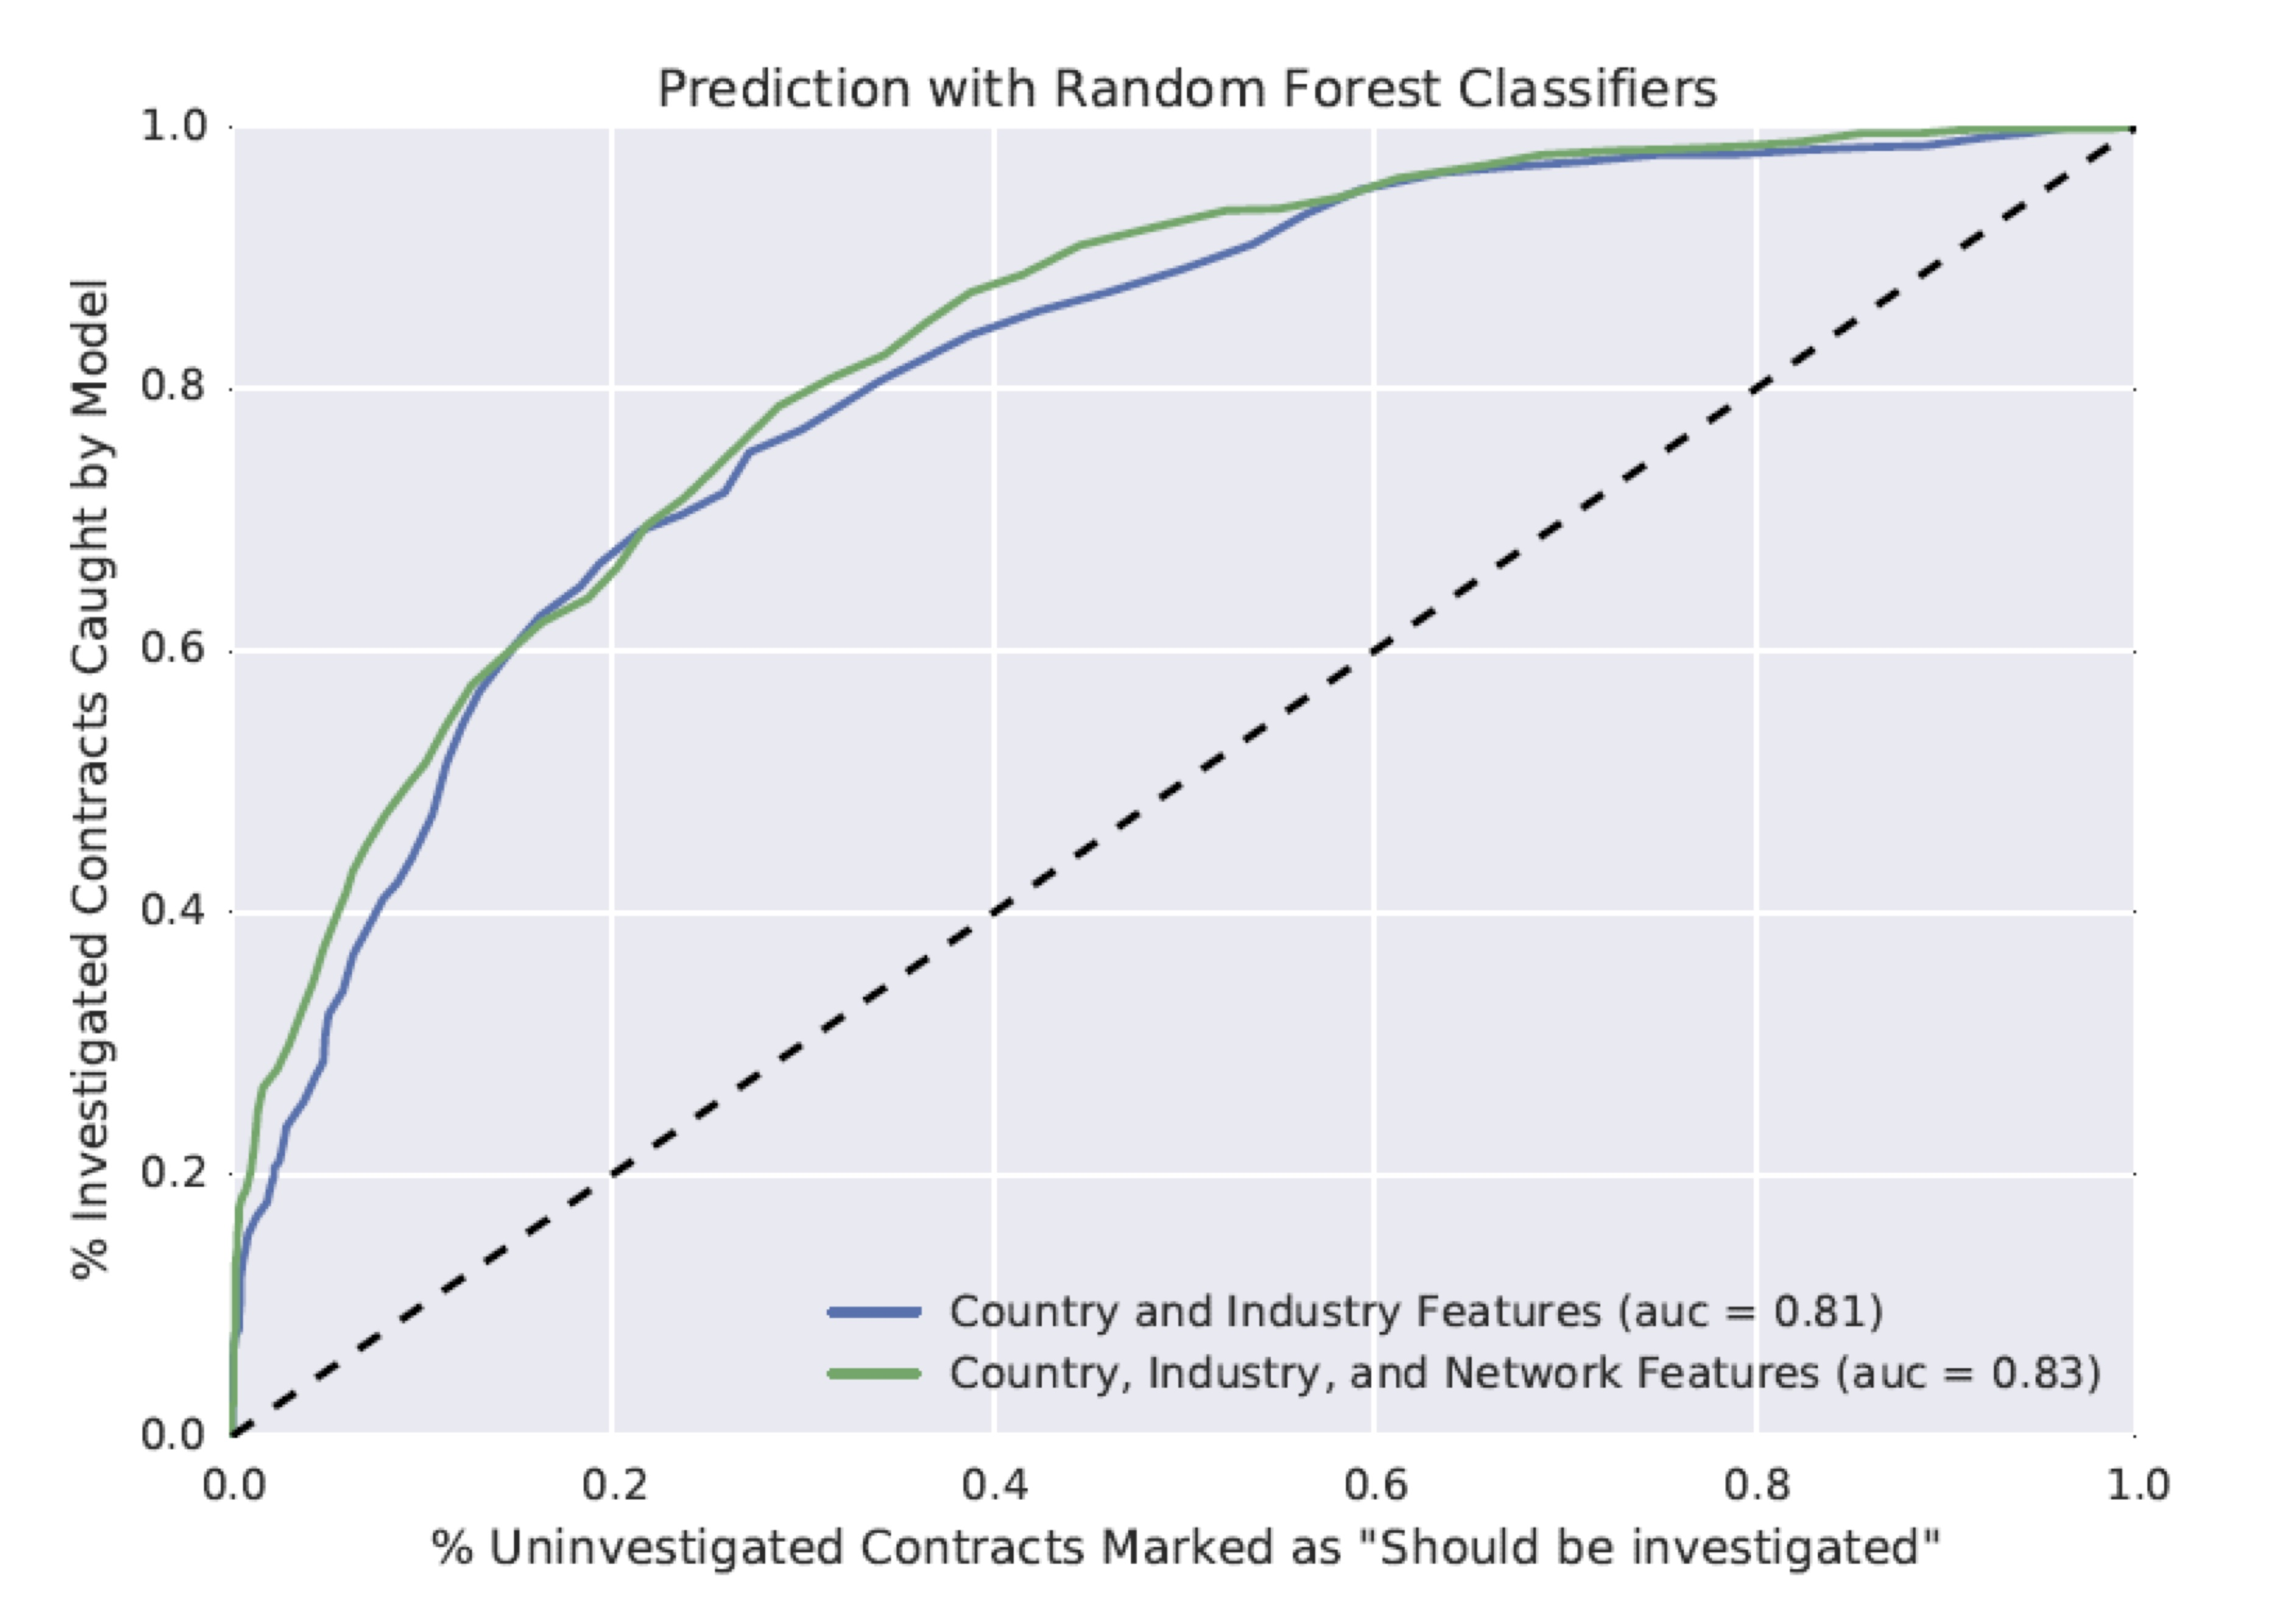
\includegraphics[width=1.05\textwidth,keepaspectratio]{../img/roc.jpg}
\end{center}
\noindent \footnotesize{\textbf{Source:} Own creation.}
\end{figure}


\section{Web visualization application: dashboard} \label{sec_visual}

In order for the investigators at the World Bank to look for suspicions patterns of corruption, collusion and fraud in their procurement data in a proactive way and not by waiting for whistle-blowers to alert them about potential  problems in the procurements process and, also, to use the classification model to target their investigations to the entities, projects and contracts that have higher risk of being a substantiated case if investigated, in this project we created a web application that helps them do their work. That tab helps them get to get the sense of the kind of patters to look for in the data.


Figure \ref{fig_dashboard} shows a visualization of the dashboard created for the investigators at the Integrity Vice Presidency. As it can be seen from the image, the dashboard has four main tabs, About, Country and Supplier\footnote{The tab Contact is just a way for them to contact us in case of any error in the app.}. Each tab has a specific purpose that might help the investigators perform more proactive investigations. To start, the About tab shows a brief summary of how to use the app. It displays some examples of what can it be considered a red flag in the process of searching for possible corruption, collusion and/or fraud in the procurement data. It actually refers to figure \ref{fig_what_corr} in page \pageref{fig_what_corr}.

\begin{figure}[H]
\begin{center}
\caption{Dashboard}
\label{fig_dashboard}
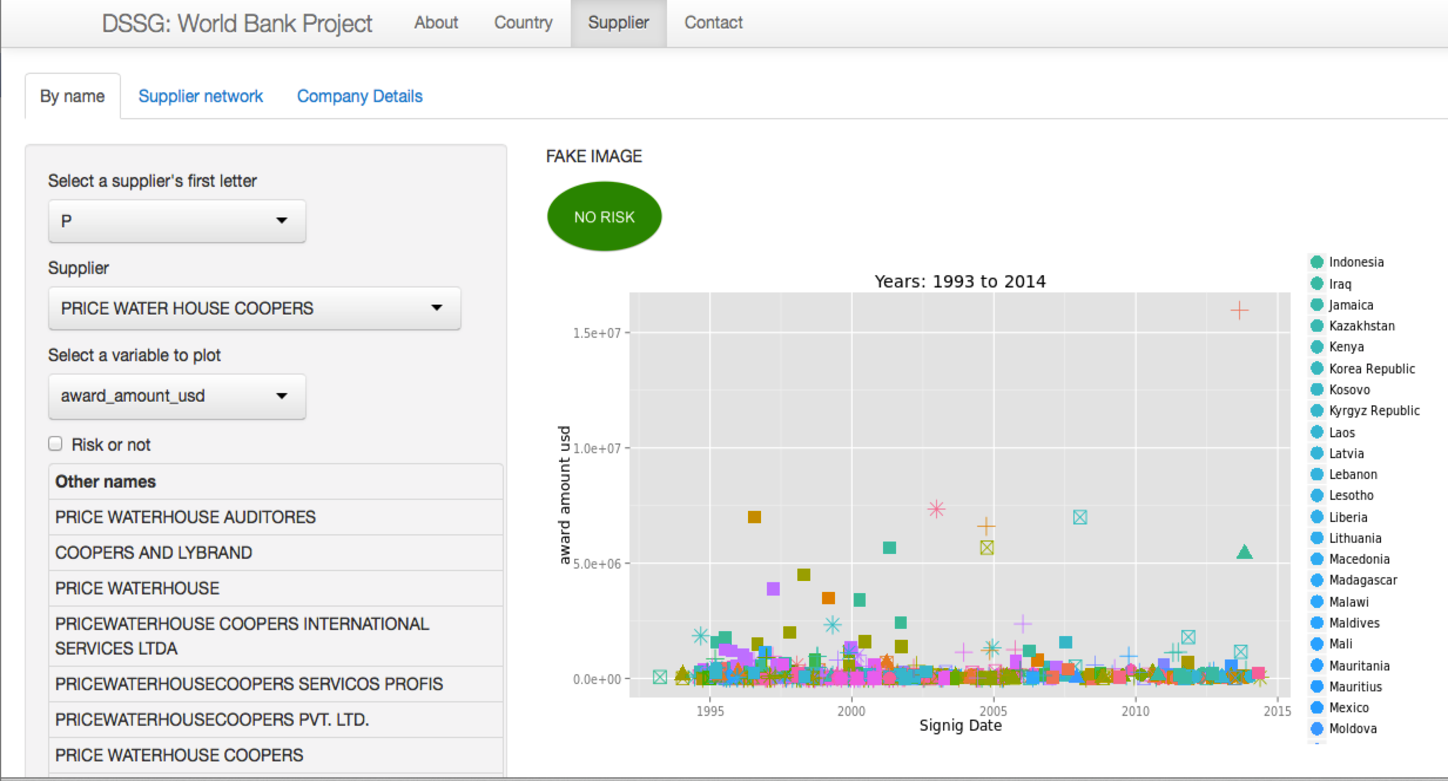
\includegraphics[width=1.05\textwidth,keepaspectratio]{../img/dashboard.pdf}
\end{center}
\noindent \footnotesize{\textbf{Source:} Own creation.}
\end{figure}


\subsection{County tab: Red-flags from data}

After that, the \textit{County tab} is designed to actually look for those red flags presented on the About tab but in real data form the historic and major awards as well as the investigations data. As chapter \ref{chap_procurements} presented figure \ref{fig_what_corr} suggesting ideas of how to look for common patterns to identify potential cases of corruption, collusion, fraud, coercion and other types of malicious behavior among the procurements that the World Bank gives to countries all over the world. The objective of this tab is to try to replicate those figures by using real data in order to provide a valuable insight to the investigators working in the Integrity Vice Presidency to help them attack this problem.

For example, this tab shows images such as \ref{fig_mex-top15} and \ref{fig_mex-amount}. To start, figure  \ref{fig_mex-top15}shows possible cases of collusion in Mexico. It shows the top 15 contractors in terms of awarded amount. Figure tries to replicate figure \ref{fig_cum_value} by showing that that only few contractors are getting almost all the contracts, as much as 30\% in Mexico and actually it's going only to few states.
% \begin{figure}[H]
% \begin{center}
% \caption{Red Flags: top 15 contracts in Mexico}
% \label{fig_mex-many}
% 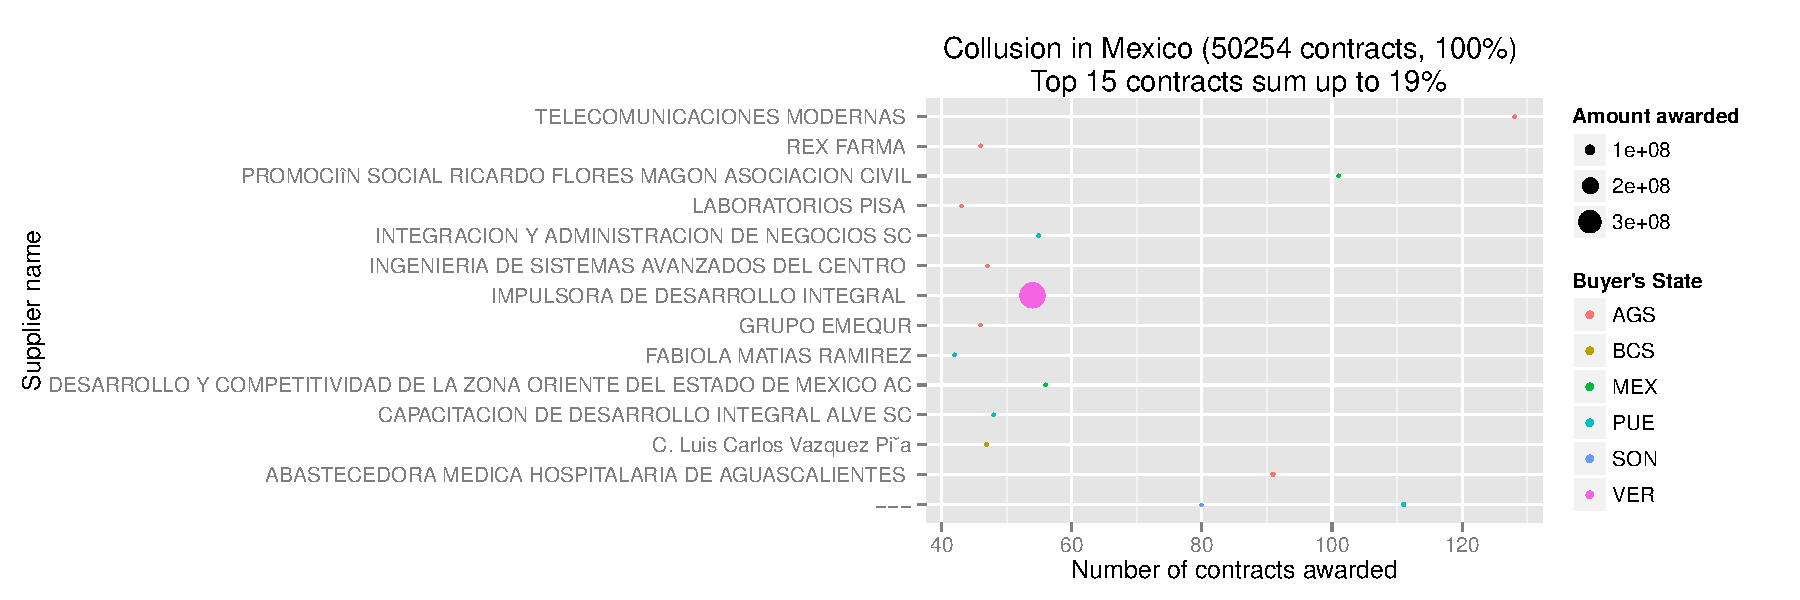
\includegraphics[width=1.05\textwidth,keepaspectratio]{../img/mex_many-15.pdf}
% \end{center}
% \noindent \footnotesize{\textbf{Source:} Own creation.}
% \end{figure}
\begin{figure}[H]
\begin{center}
\caption{Red Flags: top 15 contracts in Mexico}
\label{fig_mex-top15}
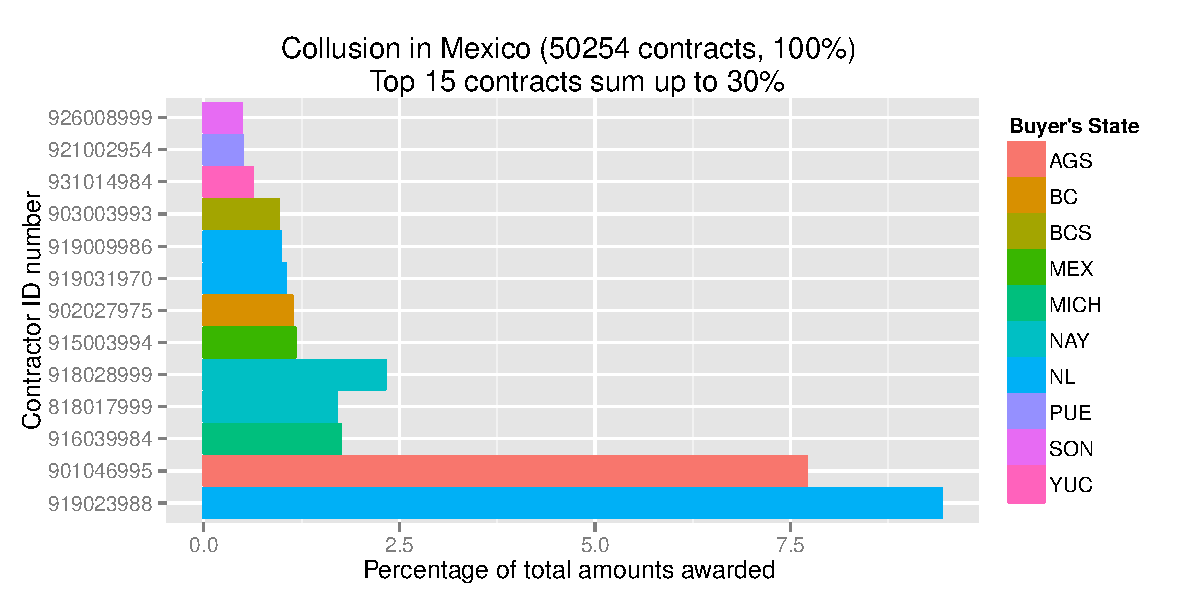
\includegraphics[width=1.05\textwidth,keepaspectratio]{../img/mex-top-15.pdf}
\end{center}
\noindent \footnotesize{\textbf{Source:} Own creation.}
\end{figure}


Then, figure \ref{fig_mex-amount} shows the distribution of number of contracts against the awarded amount per supplier and colored by the State. This figure helps them to identify outlier in the procurements. It shows that, as expected, there are few contractors that are receiving contracts with very big awarded amounts in USD against suppliers that are receiving a considerable bigger amount of small contracts compared to the majority of the suppliers. This might or might not be indicators of corruption, collusion or fraud, but helps the investigators to identify what suppliers are receiving more in terms of money or contracts such that they can  keep closer attention.


\begin{figure}[H]
\begin{center}
\caption{Red Flags: Outliers in Mexico}
\label{fig_mex-amount}
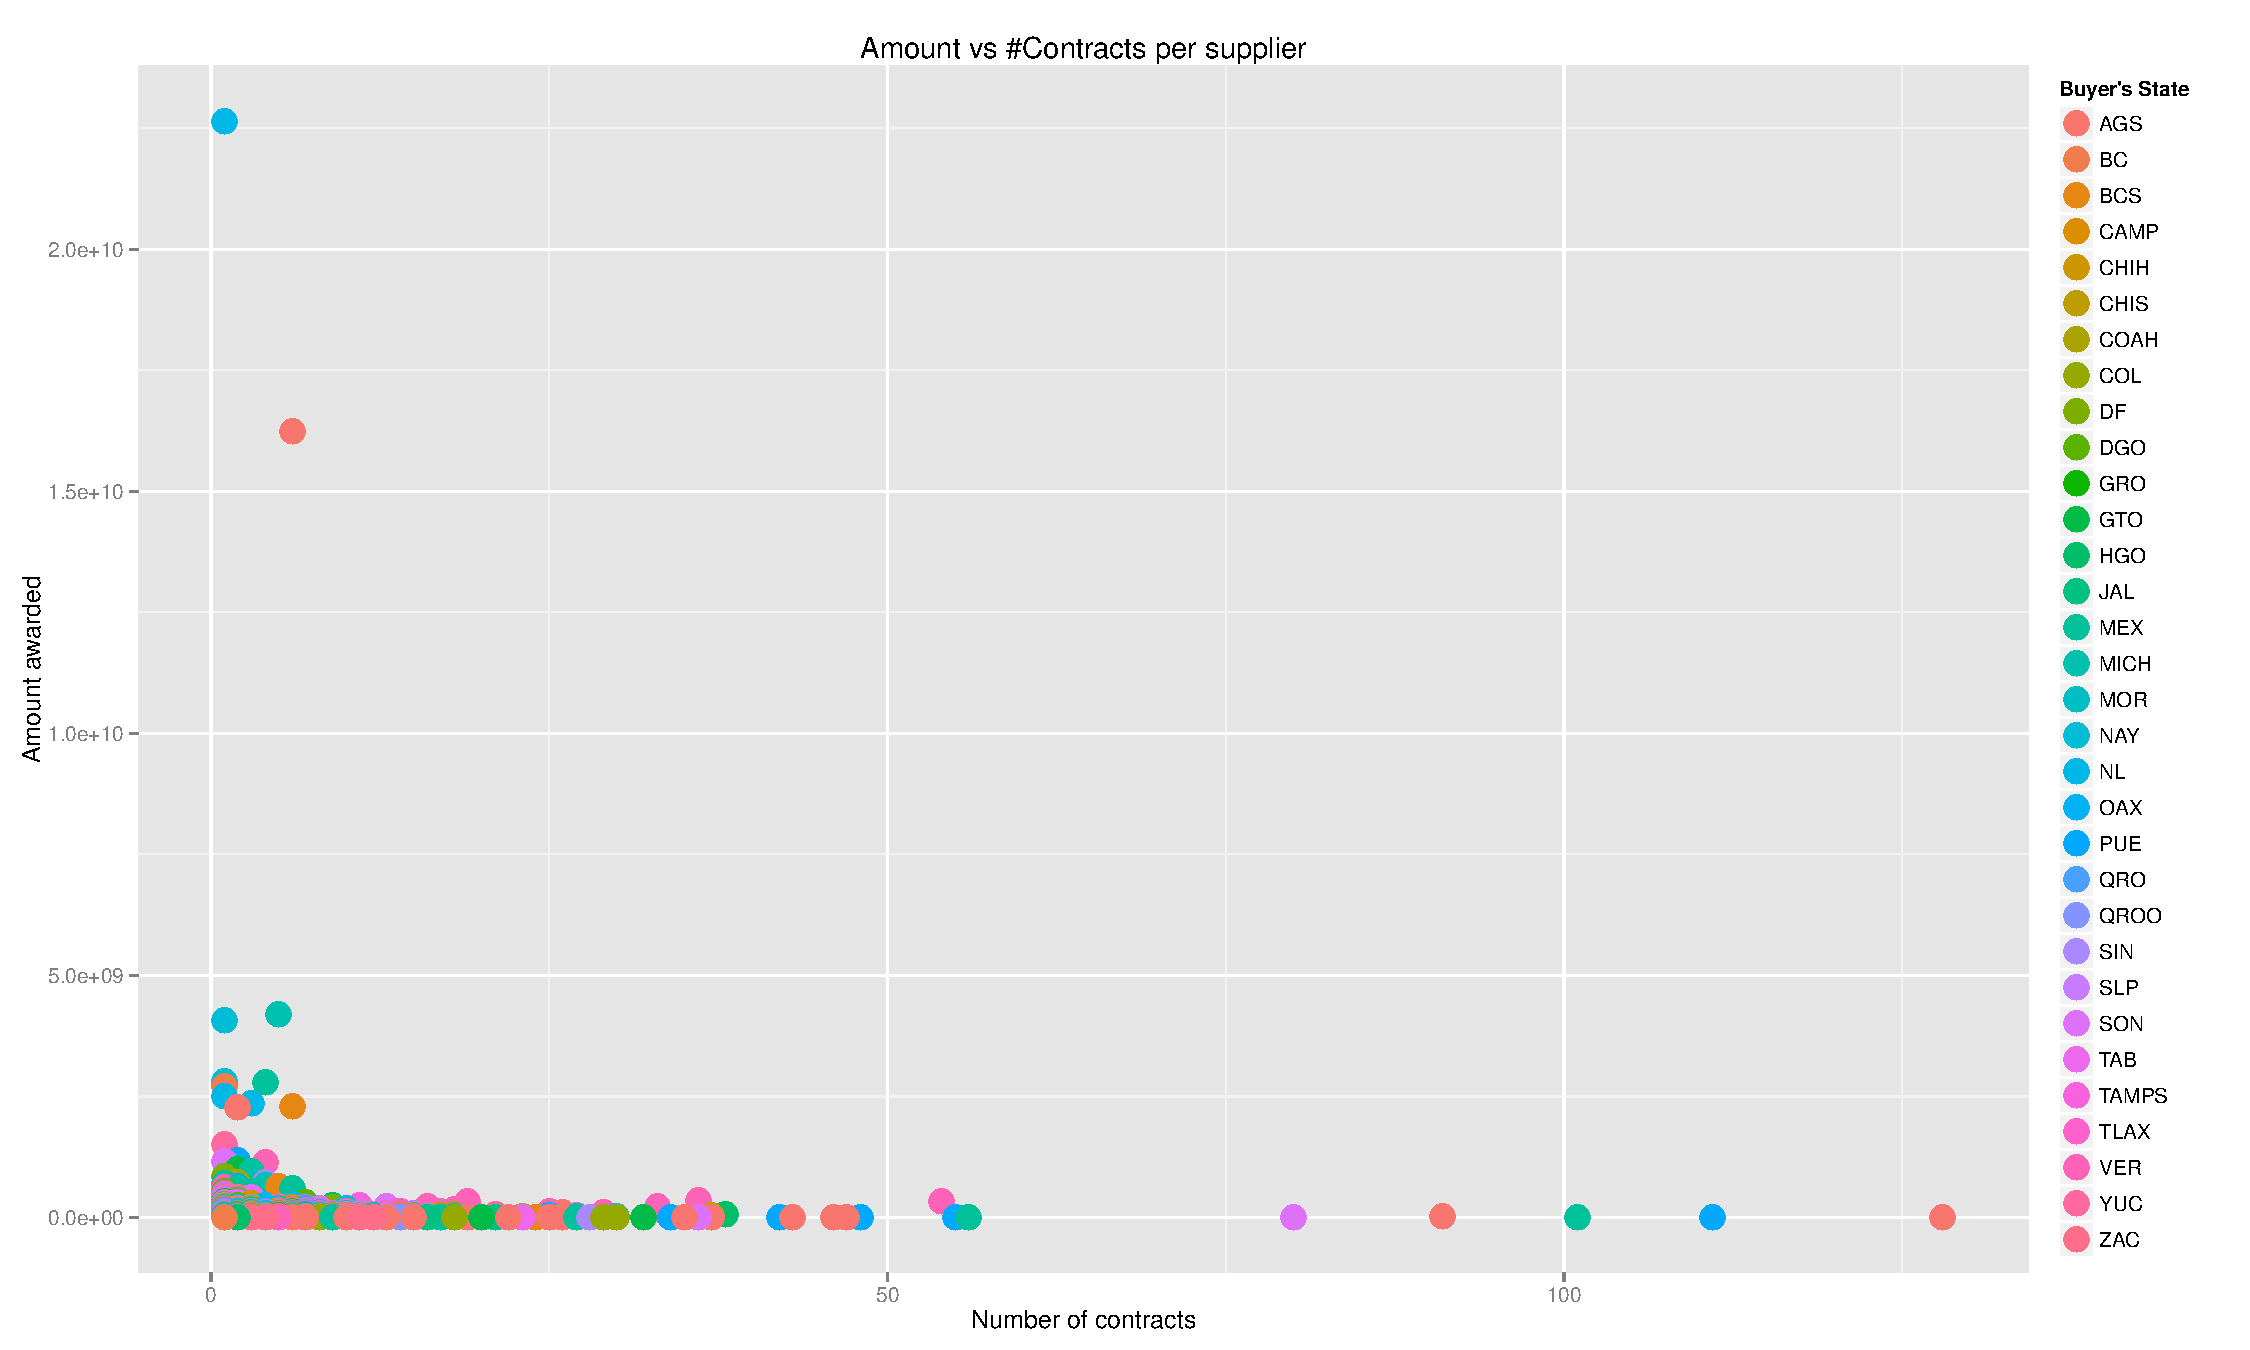
\includegraphics[width=1.05\textwidth,keepaspectratio]{../img/mex-amount-contract.pdf}
\end{center}
\noindent \footnotesize{\textbf{Source:} Own creation.}
\end{figure}

\subsection{Supplier tab: Name disambiguation, model \& network}

The next tab in the dashboard is the \textit{Supplier tab} which is the most relevant because it displays the result of the model and the one displayed at figure \ref{fig_dashboard}. In this tab the investigators at the World Bank can select a specific entity to look at. For example, figure \ref{fig_dashboard} shows the case of Price Waterhouse Coopers. The first thing to notice is that the dashboard displays a long list of names under the `Other names' subtitle. Those names show the results of the Google search algorithm, i.e. all the other names by which an investigator might find the entity Price Waterhouse Coppers among the different databases form the World Bank. The list can be downloaded for future reference. This tab also shows a plot to display any of the desired numeric variable against time  for that specific contractor and colored by country so that investigators can look for suspicious patters.

Maybe the most important part of this tab and the dashboard is the \textit{Risk factor icon}. As it can be seen from figure \ref{fig_dashboard}, after the investigator has selected an entity, the dashboard displays an icon that represent the level of risk that entity has in the random forest. This is the most valuable item in the dashboard because if it helps the investigator to confirm whether their suspiciousness for an entity is solid enough for them to take action into a deeper investigation. There are three categories for risk that include: no risk, low risk and high risk. The classification in those categories was very conservative so that it helps them to identify cases that require major attention. The figure \ref{fig_risk_map} is an static image that shows the risk factor among the World. It summarizes the results of the model and the risk item shown in the dashboard.

\subsubsection{Contract specific risk map}

\begin{figure}[H]
\begin{center}
\caption{Risk map (Sample)}
\label{fig_risk_map}
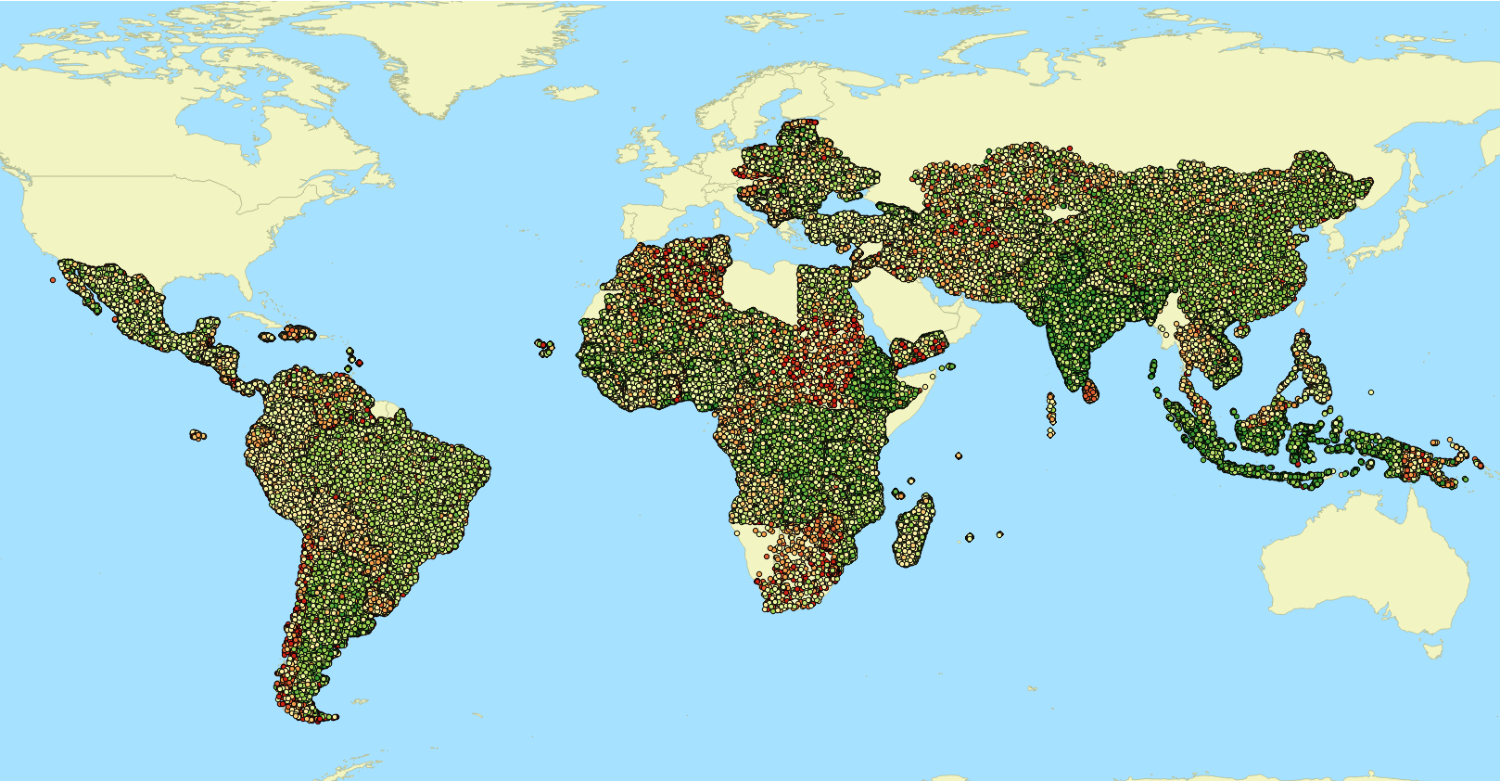
\includegraphics[width=\textwidth,height=1\textheight,keepaspectratio]{../img/risk_map.pdf}
\end{center}
\noindent \footnotesize{\textbf{Source:} Own creation based on \cite{wb_i_map}. \\Data from the World Bank \parencite{wb_data}.}
\end{figure}



After that, the sub tab \textit{Supplier network} shows the one degree co-award live network for the entity selected. Figure \ref{fig_network} is an example of what this tab shows. In this tab the user can also download the data from the network for future reference along with the data from the neighbors that where investigated.

Finally, sub tab \textit{Company details} shows all the data available to download referring to the entity selected in the previous tab so that explore with detail each one of the projects where the entity participated. It includes data for the projects awarded and not awarded but where it participated as a bidder, which might help them to identify collusion or coercion.

\subsection{Interactive map}

Finally, there is a second visualization created for the investigators at the World Bank, an interactive map that shows the evolution of the contracts in time. This visualization was developed in collaboration of the participants of the Data sprint hackathon organized with the World Bank. There is a public version available at \href{http://detecting-corruption.carlospetricioli.com/interactive_map}{detecting-corruption.carlospetricioli.com/interactive\_map}. The map displays how contracts accumulate in time among the countries to which the World Bank gives contracts to. The color correspond to the sector in the project. If you point to any of countries, the visualization displays the amount borrowed and supplied from/to that country. If you click on any of the flying dots, which refers to a specific country and flies from the supplier country to the borrowed one, it displays the data. It includes the name of the project, the product line, the major sector, the type of procurement, the method of selection, the category, the region as well as the amount. This visualization is just one more way for the investigators to study the behavior of the contracts among the world and can be used in hand with the risk map shown in figure \ref{fig_risk_map} to identify potential risk factors.


\begin{figure}[H]
\begin{center}
\caption{Interactive map}
\label{fig_interactive_map}
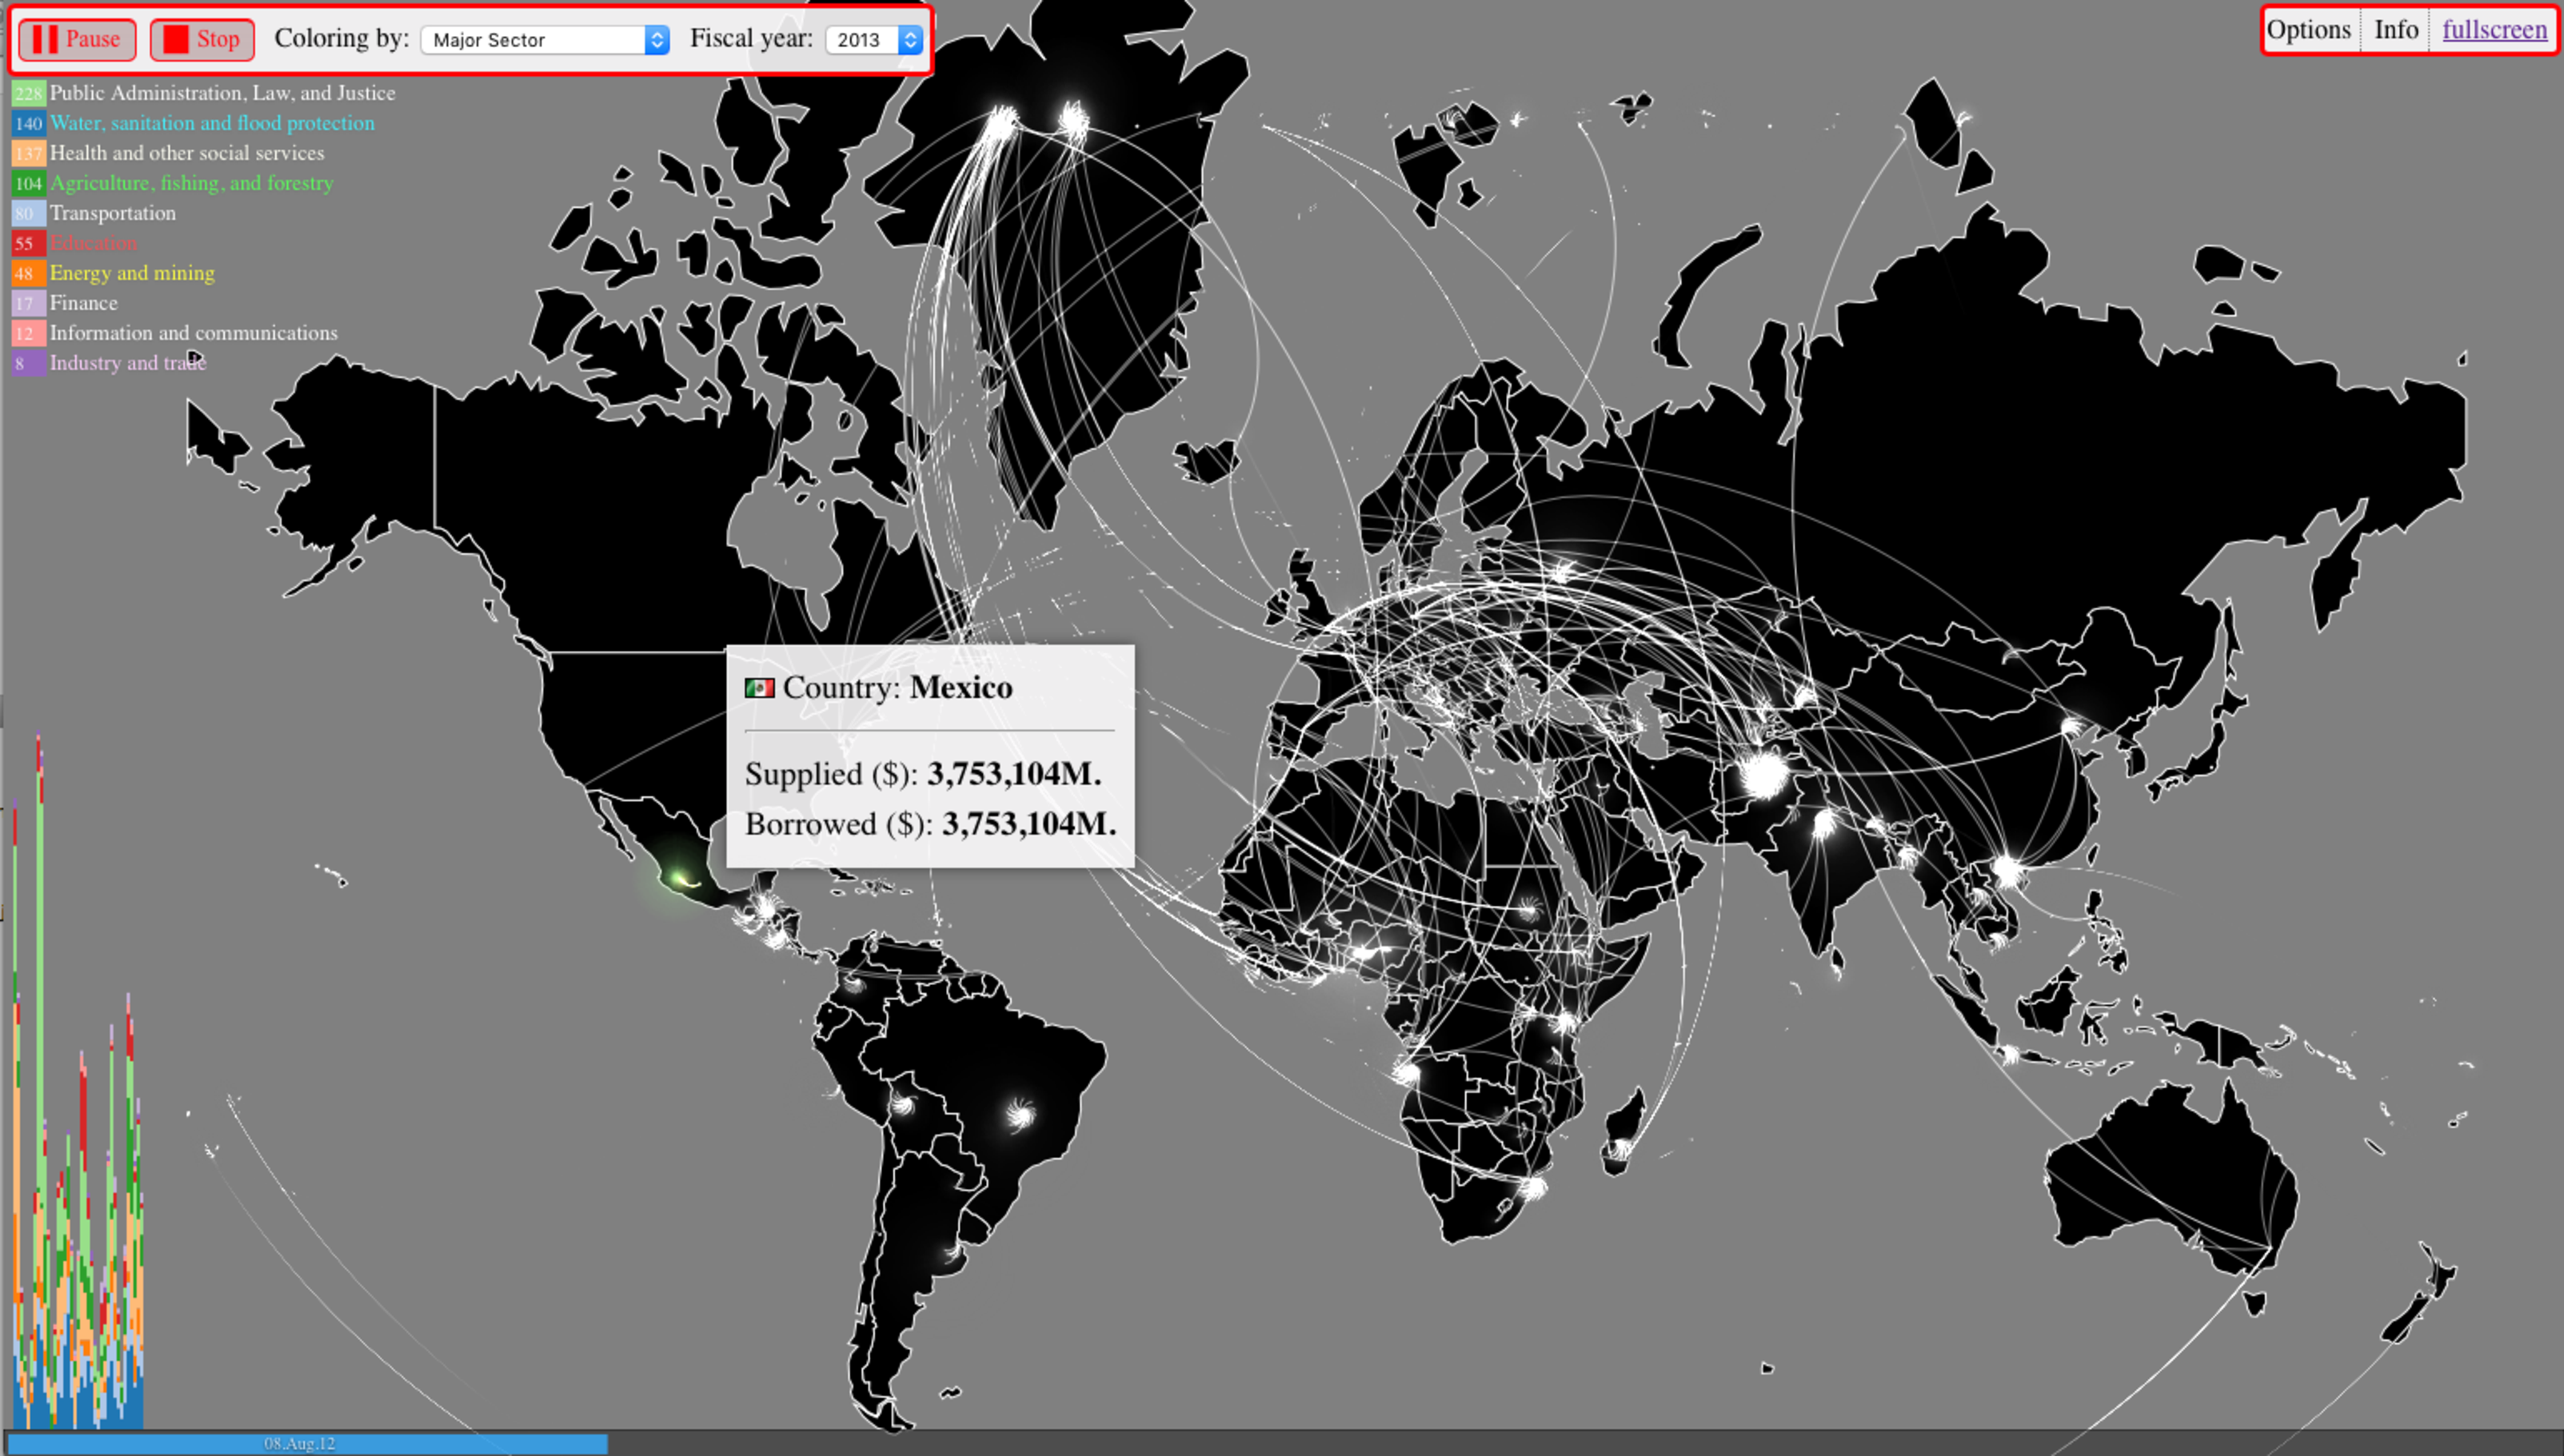
\includegraphics[width=\textwidth,height=1\textheight,keepaspectratio]{../img/interactive_map_mex.pdf}
\end{center}
\noindent \footnotesize{\textbf{Source:} Own creation based on \cite{wb_i_map}. \\Go to \href{http://detecting-corruption.carlospetricioli.com/interactive_map}{detecting-corruption.carlospetricioli.com/interactive\_map} to see a live version. \\Data from the World Bank \parencite{wb_data}.}
\end{figure}





